\documentclass[12pt, titlepage]{article}

\usepackage{booktabs}
\usepackage{tabularx}
\usepackage{hyperref}
\hypersetup{
    colorlinks,
    citecolor=black,
    filecolor=black,
    linkcolor=red,
    urlcolor=blue
}
\usepackage[round]{natbib}

%% Comments

%\usepackage{color}
\usepackage[dvipsnames]{xcolor}

\newif\ifcomments\commentstrue

\ifcomments
\newcommand{\authornote}[3]{\textcolor{#1}{[#3 ---#2]}}
\newcommand{\todo}[1]{\textcolor{red}{[TODO: #1]}}
\else
\newcommand{\authornote}[3]{}
\newcommand{\todo}[1]{}
\fi

\newcommand{\wss}[1]{\authornote{blue}{SS}{#1}}
\newcommand{\an}[1]{\authornote{magenta}{Author}{#1}}
\newcommand{\meow}[1]{\authornote{Orchid}{JG}{#1}}

%% Common Parts

\newcommand{\progname}{Kaplan}


% jen things
\usepackage{xr} % reference external documents
\externaldocument{../../SRS/SRS}
\externaldocument{../../Design/MIS/MIS}
\externaldocument{../../Design/MG/MG}
\externaldocument{../SystVnVPlan/SystVnVPlan}
\usepackage{graphicx} % for figures
\usepackage{float} % for H when placing figures
\usepackage{listings} % for code lstlisting
\usepackage{multirow} % for multirow in tables
\usepackage{chngpage} % for stretching margins around large tables
\usepackage{enumitem} % for lists with fixed string presets (set 1 set 2 etc)


\begin{document}

\title{Project Title: Unit Verification and Validation Plan for \progname{}} 
\author{Jen  Garner}
\date{\today}
	
\maketitle

\pagenumbering{roman}

\section{Revision History}

\begin{tabularx}{\textwidth}{p{3cm}p{2cm}X}
\toprule {\bf Date} & {\bf Version} & {\bf Notes}\\
\midrule
December 3rd, 2018 (Monday) & 1.0 & First draft \\
\bottomrule
\end{tabularx}

~\newpage

\tableofcontents

%\listoftables

\listoffigures

\newpage

\section{Symbols, Abbreviations and Acronyms}

\renewcommand{\arraystretch}{1.2}
\begin{tabular}{l l} 
  \toprule		
  \textbf{symbol} & \textbf{description}\\
  \midrule 
  T & Test \\
  RNS & Random Number Seed \\
  MG & Module Guide \\
  SRS & Software Requirements Specification \\
  MIS & Module Instance Specification \\
  gac & Genetic Algorithm Control (Module) \\
  CI & Continuous Integration \\
  HPC & High-performance computing \\
  pmem & population member (of ring) \\
  PEP & Python enhancement proposal (from PEP8) \\
  \bottomrule
\end{tabular}\\

\newpage

\pagenumbering{arabic}

This document provides unit testing cases for each of the modules, except where 
the module uses an external library (geometry, energy, and rmsd). The purpose 
of the document is given, as well as the scope of the covered tests. This 
document is meant to be read alongside the MIS document, since the MIS provides 
the outputs and inputs of each function and method. The tools needed to run the 
tests is discussed in Section \ref{test-tools}.

\section{General Information}

\subsection{Purpose}

This document will identify what testing is going to be done on \progname{}. 
This document is different from the System VnV Plan in that it considers each 
module as already written according to the Module Instance Specification (MIS) 
document. Since each function, method, class, and algorithm has been given, 
they can be tested using a white box approach, where the inputs, outputs, and 
transitions between the inputs and outputs are known.

\wss{Identify software that is being unit tested (verified).}

\subsection{Scope}

The Hardware-Hiding module will not be covered in this unit testing plan, since 
the developer does not have any means or the expertise needed to properly test 
such a module. As mentioned in the System VnV Plan, the energy, geometry, and 
RMSD modules will be tested by running the tests for the libraries that these 
modules import.

The most important modules to test are the two input modules: Molecule Input 
and GA Input. Since this program is likely to be run on a server with multiple 
iterations of different molecules, checking of the inputs before submission is 
very important. If the errors in setup are caught early, jobs (that cannot 
actually run) can be prevented from sitting in queues on the high-performance 
computing (HPC) clusters.

It will be important to test the Crossover \& Mutation (mutations) module, 
since this is how the solutions will evolve over time. If the new population 
members are not correctly initialized (or if they are copies of the old 
population members without any mutation), then the optimization will not work 
and running the program would have been a waste of resources and time.

The GA Input module (gac) is probably the least important module to test, since 
it is only running other modules in a sequence. Basic tests, such as: 1. was 
the Ring initialized, 2. did the Ring change as a result of running the gac 
module, 3. were the outputs and inputs called, can be done on gac if necessary.

Other modules that will be tested include: fitg, tournament, ring, pmem, and 
output.

\wss{What modules are outside of the scope.  If there are modules that are
  developed by someone else, then you would say here if you aren't planning on
  verifying them.  There may also be modules that are part of your software, but
  have a lower priority for verification than others.  If this is the case,
  explain your rationale for the ranking of module importance.}

\section{Plan}
	
\subsection{Verification and Validation Team}

Mulder, c'est moi.

\subsection{Automated Testing and Verification Tools} \label{test-tools}

The Ayers' Lab group has a linter called Cardboardlint 
\url{https://github.com/theochem/cardboardlint}. If time permits, this linter 
can be joined with Travis CI (Continuous Integration) to enable static code 
checking (for PEP8) and code coverage. Prior to enabling this linter, the 
following libraries can be added to the Travis build:

\begin{itemize}
	\item coverage
	\item pylint
	\item nosetests (also called nose)
	\item pycodestyle
	\item pydocstyle (with numpy convention)
\end{itemize}

The report generated by Travis CI will be uploaded to the VnV Report. The 
.travis.yml file will be added to the \progname{} repository so the 
installation and verification process can be monitored. Eventually the program 
will be made into a conda package itself, then a conda environment can be used 
for an easy installation process.

\wss{What tools are you using for automated testing.  Likely a unit testing
  framework and maybe a profiling tool, like ValGrind.  Other possible tools
  include a static analyzer, make, continuous integration tools, test coverage
  tools, etc.  Explain your plans for summarizing code coverage metrics.}

\subsection{Non-Testing Based Verification}

Some jupyter notebooks (\url{http://jupyter.org/}) will be made by the 
developer as a way to test the geometry module and the energy module. These 
notebooks are an easy way to ensure that the imported libraries behave as 
intended with the \progname{} code and that the developer has correctly 
interpreted the other libraries' documentation and usage. These notebooks will 
be helpful later-on as documentation, in case the user wants to manipulate the 
energy calculations and/or the parts of the geometry that are optimized.

There will be a code review with lab members Kumru Dikmenli and Xiaomin Huang 
during a weekly meeting. Once the SRS has been updated to address comments from 
Prof. Paul Ayers (supervisor), there will also be a code walk-through with the 
supervisor.

\section{Unit Test Description}

\begin{figure}[H]
	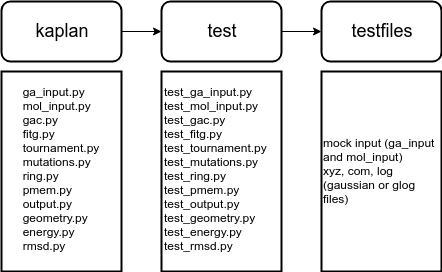
\includegraphics[width=\textwidth]{directory-structure.png}
	\caption{The directory structure for the unit testing. An arrow from A to B 
		implies that B is a subdirectory of A.}
	\label{fig-dir-struct}
\end{figure}

The directory structure for testing is as follows (see Figure 
\ref{fig-dir-struct}). First we have the \textit{kaplan} directory that 
contains the code. Within this directory, there is the \textit{test} 
subdirectory. This \textit{test} directory has a test file (.py) for each 
module. Within the \textit{test} directory there is a \textit{testfiles} 
subdirectory, which contains mostly molecule input and output, as well as 
kaplan-formatted input for the two input modules. Each test file has the naming 
convention: test\_module\_name.py and each function within each of the test 
files has the naming convention: test\_function\_name.py. If the test is for a 
class, then the naming convention for the test becomes: 
test\_Classname\_methodname.py.

\meow{I wasn't sure where to put the above information. It seems relevant to my 
	documentation. Also, I think the naming convention is actually required by 
	nosetests, but I could be wrong.}

\wss{Reference your MIS and explain your overall philosophy for test case
  selection.}

\subsection{Tests for Functional Requirements}

For many of these tests, the numpy python library testing module will be 
utilized. Within that testing module, there is an assert\_raises function. This 
function is used to ensure that the correct errors are raised for a given 
function call and function inputs.

\wss{Most of the verification will be through automated unit testing.  If
  appropriate specific modules can be verified by a non-testing based
  technique.  That can also be documented in this section.}

\subsubsection{GA Input Module} \label{test-ga_input}

\meow{I couldn't figure out how to make the mref work in this document, even 
	when the MG was added as an external document in the tex file. Any 
	suggestions?}

From Section \ref{section-ga_input} in the MIS, we have a set of unit tests for 
the GA Input Module. The purpose of these tests is to ensure that an error is 
raised if the user does one of the following:
\begin{enumerate}
	\item Provides a file name that does not exist in the given directory.
	\item Forgets to include an input parameter or misspells an input parameter.
	\item Puts the same input parameter twice or adds too many input parameters.
	\item Provides input values that do not satisfy the program constraints 
	(for example, num\_slots $<$ num\_filled).
	\item Provides input values of the wrong type (for example, num\_mevs is 
	equal to 3.2, which doesn't make physical sense).
\end{enumerate}
The tests should also confirm that correct input can pass without raising 
errors. A couple of valid and invalid input files will be available in the 
testfiles directory (see Figure \ref{fig-dir-struct}). The valid input files 
can also act as example input for instructional purposes.

\meow{I might need to add a test to see what happens when the user tries to 
open a file that they do not have read permissions for. However, I can't think 
of a reasonable case where this would happen. I'm also not sure how to create 
that error without trying to access someone else's files... I'll assume the 
interpreter error message will be sufficient.}

As per the MIS (Section \ref{section-ga_input}), there are two functions within 
the ga\_input module: read\_ga\_input, which checks the number of inputs and 
ensures the file can be opened (file exists), and verify\_ga\_input, which 
checks that all of the input parameters have been given and that their values 
are of the right type and within the necessary bounds.

\wss{Include a blurb here to explain why the subsections below cover the module.
  References to the MIS would be good.  You will want tests from a black box
  perspective and from a white box perspective.  Explain to the reader how the
  tests were selected.}

\begin{enumerate}

\item{test\_read\_ga\_input\\}

Type: automatic
					
Initial State: None
					
Input: 

\begin{table}[H]
	\begin{tabular}{ccp{4cm}}
		\toprule
		file name & error raised & test covered \\
		\midrule
		example\_ga\_input\_file.txt & None & good input does not raise an 
		error \\
		example2\_ga\_input\_file.txt & None & good input can have extra 
		whitespace and is impervious to capitalization \\
		no-such-file & FileNotFoundError & file does not exist and therefore 
		cannot (and should not) be opened \\
		bad1\_ga\_input\_file.txt & ValueError & num\_mevs appears twice (too 
		many input parameters) \\
		bad2\_ga\_input\_file.txt & ValueError & num\_atoms is not in the input 
		file (missing input parameter) \\
	\end{tabular}
\end{table}
					
Output: None

Test Case Derivation: None

How test will be performed: If the read\_ga\_input function can be called with 
the good input files without raising an error, then the test is assumed to 
pass. Conversely, if the bad inputs raise the expected error as per the 
assert\_raises function, then the test will pass.
					
\item{test\_verify\_ga\_input\\}

Type: automatic
					
Initial State: None
					
Input:

\begin{table}[H]
	\begin{tabularx}{\textwidth}{p{5cm}p{3cm}p{6.5cm}}
		\toprule
		file name or & \multirow{2}{*}{error raised} & \multirow{2}{*}{test 
		covered} \\
		change in ga\_input\_dict*& & \\
		\midrule
		example\_ga\_input\_file.txt & None & good input does not raise an 
		error \\
		example2\_ga\_input\_file.txt & None & good input can have extra 
		whitespace and is impervious to capitalization \\
		bad3\_ga\_input\_file.txt & ValueError & num\_geoms is spelt wrong 
		(input file does not contain all of the expected parameters) \\
		num\_slots = -1 & AssertionError & num\_slots must be positive \\
		num\_filled = 150 & AssertionError & num\_filled must be $\leq$ 
		num\_slots \\
		num\_mevs = -300 & AssertionError & num\_mevs must be positive \\
		num\_swaps = 20 & AssertionError & num\_swaps must be $\leq$ num\_geoms 
		\\
		num\_muts = 30 & AssertionError & num\_muts must be $\leq$ num\_atoms-3 
		\\
		num\_geoms = -2 & AssertionError & num\_geoms must be positive \\
		num\_atoms = 2 & AssertionError & num\_atoms must be $\geq$ 4 \\
		fit\_form = 1 & AssertionError & fit\_form will only be implemented 
		with one function initially; only fit\_form = 0 is accepted \\
		pmem\_dist = 57 & AssertionError & pmem\_dist has to be $\leq$ 
		1/2*num\_slots (rounded down) \\
		coef\_energy = -5 & AssertionError & coef\_energy must be positive \\
		coef\_rmsd = -5 & AssertionError & coef\_rmsd must be positive \\
		t\_size = 25 & AssertionError & t\_size must be $\leq$ num\_filled \\
	\end{tabularx}
\end{table}

\noindent * for changes to the ga\_input\_dict, the other parameters are based 
on the contents of the example\_ga\_input\_file.txt, where we have:
\begin{lstlisting}[language=python, showstringspaces=false]
ga_input_dict = {`num_mevs': `1000', `num_slots': `100',
		 `num_filled': `20', `num_geoms': `3',
		 `num_atoms': `10', `t_size': `7',
		 `num_muts': `3', `num_swaps': `1',
		 `pmem_dist': `5', `fit_form': `0',
		 `coef_energy': `0.5', `coef_rmsd': `0.5'}
\end{lstlisting}
					
Output: None

Test Case Derivation: None

How test will be performed: as with the tests for read\_ga\_input, these tests 
will use the numpy.testing assert\_raises function to ensure that the correct 
errors are raised. The verify\_ga\_input function is also responsible for 
checking the types of the input; if a value (for example, num\_geoms) is 
supposed to be an integer and python cannot convert the input to an integer, 
then an error will be raised. This is not covered by the unit tests, since it 
is assumed that trying to use incorrect types (a string as an integer) will 
yield an obvious error.
    
\end{enumerate}

\subsubsection{Molecule Input Module}

The mol\_input module will be tested in a similar fashion to the 
ga\_input\_module (Section \ref{test-ga_input}), with the added tests as needed 
to check the input geometry, QCM, and BS. As per the module uses hierarchy in 
the module guide document, the mol\_input module uses the geometry and energy 
modules. Therefore, to test this module properly, both of these other modules 
must be adequately tested as well.

\wss{Include a blurb here to explain why the subsections below cover the module.
	References to the MIS would be good.  You will want tests from a black box
	perspective and from a white box perspective.  Explain to the reader how the
	tests were selected.}

\begin{enumerate}
	
\item{test\_read\_mol\_input\\}

Type: automatic

Initial State: None

Input: 
	
\begin{table}[H]
	\begin{tabular}{ccp{4cm}}
		\toprule
		file name & error raised & test covered \\
		\midrule
		example\_mol\_input\_file.txt & None & good input does not raise an 
		error \\
		example2\_mol\_input\_file.txt & None & good input can have extra 
		whitespace and is impervious to capitalization \\
		no-such-file & FileNotFoundError & file does not exist and therefore 
		cannot (and should not) be opened \\
		bad1\_mol\_input\_file.txt & ValueError & qcm appears twice (too 
		many input parameters) \\
		bad2\_mol\_input\_file.txt & ValueError & struct\_type is not in the 
		input file (missing input parameter) \\
	\end{tabular}
\end{table}
	
Output: None

Test Case Derivation: None

How test will be performed: numpy.testing.assert\_raises.

\item{test\_verify\_mol\_input\\}

Type: automatic

Initial State: None

Input:

\begin{table}[H]
	\begin{tabularx}{\textwidth}{p{5cm}p{3cm}p{6.5cm}}
		\toprule
		file name or & \multirow{2}{*}{error raised} & \multirow{2}{*}{test 
			covered} \\
		change in mol\_input\_dict*& & \\
		\midrule
		example\_mol\_input\_file.txt & None & good input does not raise an 
		error \\
		example2\_mol\_input\_file.txt & None & good input can have extra 
		whitespace and is impervious to capitalization \\
		bad3\_mol\_input\_file.txt & ValueError & struct\_input is spelt wrong 
		(input file does not contain all of the expected parameters) \\
		qcm = ``not-a-method" & ValueError & qcm must be available in the 
		chosen program \\
		basis = ``not-a-basis" & ValueError & basis must be available in the 
		chosen program \\
		struct\_input = ``very-bad-smiles-string" & ValueError & SMILES string 
		must be valid \\
		struct\_type = ``not-an-option" & AssertionError & struct\_type must be 
		one of: ``com", ``glog", ``xyz", ``smiles", ``name", or ``cid" \\
		prog = ``unavailable-prog" & AssertionError & prog must equal ``psi4" \\
		charge = ``0.34" & ValueError & charge must be an integer \\
		multip = -2 & AssertionError & multiplicity must be $\geq$ 0 \\
	\end{tabularx}
\end{table}

\noindent * for changes to the mol\_input\_dict, the other parameters are based 
on the contents of the example\_mol\_input\_file.txt, where we have:
\begin{lstlisting}[language=python, showstringspaces=false]
mol_input_dict = {`qcm': `hf', `basis': `sto-3g',
                  `struct_input': `C=CC=C',
                  `struct_type': `smiles', `prog': `psi4',
                  `charge': `0', `multip': `1'}
\end{lstlisting}

Output: None

Test Case Derivation: None

How test will be performed: numpy.testing.assert\_raises.
	
\end{enumerate}

\subsubsection{GA Control Module}

\wss{Include a blurb here to explain why the subsections below cover the module.
	References to the MIS would be good.  You will want tests from a black box
	perspective and from a white box perspective.  Explain to the reader how the
	tests were selected.}

\begin{enumerate}
	
\item{test\_run\_kaplan\\}

Type: automatic

Initial State: None

Input: the run\_kaplan function will be tested with two sets of inputs, one 
from example\_ga\_input\_file.txt and example\_mol\_input\_file.txt and the 
other from example2\_ga\_input\_file.txt and example2\_mol\_input\_file.txt. 
The contents of these two files can be seen below. Both sets of files are 
examples of good inputs. Note: the contents below has already passed 
verification and therefore the floating point and integer numbers are no longer 
strings.

\begin{lstlisting}[language=python, showstringspaces=false]
{`num_mevs': 1000, `num_slots': 100, `num_filled': 20,
`num_geoms': 3, `num_atoms': 10, `t_size': 7,
`num_muts': 3, `num_swaps': 1, `pmem_dist': 5,
`fit_form': 0, `coef_energy': 0.5, `coef_rmsd': 0.5}
{`qcm': `hf', `basis': `sto-3g',
`struct_input': `C=CC=C', `struct_type': `smiles',
`prog': `psi4', `charge': 0, `multip': 1}

{`num_mevs': 500, `num_slots': 50, `num_filled': 10,
`num_geoms': 2, `num_atoms': 21, `t_size': 5,
`num_muts': 5, `num_swaps': 0, `pmem_dist': 24,
`fit_form': 0, 'coef_energy': 0.75, `coef_rmsd': 0.25}
{`qcm': `hf', `basis': `sto-3g',
`struct_input': `caffeine', `struct_type': `name',
`prog': `psi4', `charge': 0, `multip': 1}
\end{lstlisting}

Output: None

Test Case Derivation: None

How test will be performed: This test will call run\_kaplan with the two sets 
of inputs. For each set of input, assert that an output file was generated, and 
that the final ring has population members (pmems) in it with non-zero age. 
Since it is impossible for all of the pmems to be generated in the last 
tournament, then at least one pmem must have an age greater than zero.

This test may require updating in the future if extinction operators are added 
to the ring. Since the extinction operators kill off a certain number of pmems, 
if a refill of the ring is called at the last mating event, then it will be 
difficult to tell if the ring has undergone any changes as a result of the 
optimization (since all pmems would then have 0 age). In this case, it might be 
possible to keep track of when a refill is triggered and assert that there if a 
pmem with non-zero age, given that a refill was not performed on the last 
mating event.
	
\end{enumerate}

\subsubsection{$Fit_G$ Module}

From the MIS document in Section \ref{section-fitg}, there are 3 access 
routines for the $Fit_G$ module: sum\_energies, sum\_rmsds, and calc\_fitness. 
There is one local function (a generator called all\_pairs\_gen) that is used 
by the sum\_rmsds function. Since this is a local function, it cannot be 
tested. However, the tests for sum\_rmsds should be thorough to ensure that the 
local function works as intended.

As per Table \ref{TblOutputVar} in the SRS document, the fitness function 
should return a positive value. The coef\_energy and coef\_rmsd values must be 
positive (which is checked by the ga\_input module). The only case where the 
answer might be negative is if the fit\_form included a logarithm (since log(n) 
< 0 for n < 1). The only fit\_form in use is a simple linear combination and 
therefore cannot be negative (unless the functions do not behave as intended).

The calc\_fitness function is trivial to test, since the sum\_energy and 
sum\_rmsd values can be fixed. All that should be tested is that the number 
returned is as calculated by hand. 

The cases where the sum\_rmsds returns zero would be easy to test, as the 
inputs would include a single geometry copied multiple times. It would also be 
easy to test the returned value of the rmsd calculation with two dissimilar 
geometries. However, checking that all possible pairs were calculated and 
summed may require a spreadsheet or jupyter notebook to properly test. A test 
should also be done to ensure that two geometries rotated and/or translated in 
space return an rmsd of zero. Of course, the value actually returned will be 
non-zero (rounding error and floating point imprecision), but it should be zero 
within a very small tolerance. This last test is not as important, as it is 
covered by the rmsd package tests already.

For the energy tests, it would require running psi4 externally and summing the 
energies for a set of geometries. Once this setup has been done, then the test 
can be automated by simple assertion that the calculated value is equal to the 
expected value for fitness.

If the program used to calculate energies or rmsd values is changed or the 
fit\_form is changed, then more tests would be required to ensure that the 
correct output is calculated by the $Fit_G$ module. However, these outputs 
should be similar and should be somewhat robust within an arbitrarily small 
tolerance.

These tests will not have the same requirements as the inputs to \progname{}, 
as it is still meaningful to calculate energies for molecules of less than 4 
atoms. Since energy calculations for smaller molecules run more quickly, then 
molecular hydrogen can be used for the tests with varying bond lengths. 

\wss{Include a blurb here to explain why the subsections below cover the module.
	References to the MIS would be good.  You will want tests from a black box
	perspective and from a white box perspective.  Explain to the reader how the
	tests were selected.}

\begin{enumerate}
	
\item{test\_sum\_energies\\}

Type: automatic (after manual calculations have been performed)

Initial State: None

Input: molecular hydrogen ($H_2$) with 5 bond lengths, with charge = 0, 
multip = 1, method = ``hf", and basis = ``sto-3g".

\begin{table}[H]
	\begin{adjustwidth}{-0.5in}{-0.5in}
	\begin{center}
	\begin{tabular}{p{4cm}p{3cm}p{8cm}}
		\toprule
		test covered & files involved & description \\
		\midrule
		energy summation is correct and positive & H2-1A.xyz, H2-2A.xyz, 
		H2-3A.xyz, H2-4A.xyz, H2-5A.xyz & assert that energy returned is 
		positive and equal to the magnitude calculated using psi4 outside of 
		\progname{} \\
	\end{tabular}
	\end{center}
	\end{adjustwidth}
\end{table}

Output: 

From the jupyter notebook using psi4 to calculate energies of 5 geometries of 
molecular hydrogen, we have (starting with 1\AA{} up to 5\AA):

\begin{lstlisting}[language=python, showstringspaces=false]
energies = [-1.0661355651335753, -0.7839052304170298,
            -0.6561980302276855, -0.6150178744908754,
            -0.5991720784780843]
abs(sum(energies)) = 3.7204287787472503
\end{lstlisting}

Test Case Derivation: None

How test will be performed: 

This work has been summarized in a jupyter notebook. The test will be written 
in a file that asserts the values from the notebook are equal to the calculated 
values from the \progname{} code.

\item{test\_sum\_rmsds\\}

Type: automatic (after manual calculations have been performed)

Initial State: None

Input: molecular hydrogen ($H_2$) with 5 bond lengths, with one geometry that 
has been translated and rotated in space.

\begin{table}[H]
	\begin{adjustwidth}{-0.5in}{-0.5in}
		\begin{center}
			\begin{tabular}{p{4cm}p{3cm}p{8cm}}
				\toprule
				test covered & files involved & description \\
				\midrule
				same geometry twice & H2-1A.xyz (twice) & run sum\_rmsds and 
				assert that rmsd is close to zero \\
				same geometry translated and rotated & H2-1A.xyz, 
				H2-1A-transrot.xyz & run sum\_rmsds and assert that rmsd is 
				close to zero \\
				all pairs are picked & H2-1A.xyz, H2-2A.xyz, H2-3A.xyz, 
				H2-4A.xyz, H2-5A.xyz & run sum\_rmsds and assert that 
				calculated rmsd is as calculated by hand \\
			\end{tabular}
		\end{center}
	\end{adjustwidth}
\end{table}


Output:

The answer for sum\_rmsds for $H_2$ 1\AA{} through to 5\AA{} is: 
14.142135623730953. Comparing the rmsd of the rotated and translated $H_2$ with 
the regular $H_2$ of the same bond length should give an rmsd of 0, as should 
the comparison between two of the same input file.

Test Case Derivation:

From the RMSD formula (see Section \ref{sec_gendef} of the SRS), the number of 
atoms in molecular hydrogen is 2, so we have:

\begin{adjustwidth}{-1in}{-1in}
	\begin{center}
		$RMSD = 
		\sqrt{\frac{1}{2}((x_{11}-x_{12})^2+(y_{11}-y_{12})^2+(z_{11}-z_{12})^2+(x_{21}-x_{22})^2+(y_{21}-y_{22})^2+(z_{21}-z_{22})^2)}$
		
		$RMSD = 
		\sqrt{\frac{1}{2}((0-0)^2+(0-0)^2+(0-0)^2+(1-2)^2+(0-0)^2+(0-0)^2)}$
		
		$RMSD = \sqrt{\frac{1}{2}((1-2)^2)}$
	\end{center}
\end{adjustwidth}

which gives the square-root of 1/2 = 0.707106781

For increasing bond length, the RMSD changes by $\sqrt{\frac{1}{2}*(g-h)^2}$, 
where g is the bond length of the first set of xyz coordinates and h is the 
bond length of the second set of xyz coordinates.

How test will be performed: 

See the jupyter notebook for more details on how to get the rmsd values using 
the rmsd package. The output from this notebook will be compared to the output 
of the code for the same input files.

\item{test\_calc\_fitness\\}

The tests for this function are already included in the System VnV Plan, in 
Section \ref{syst-vnv-calcs}.
	
\end{enumerate}

\subsubsection{Tournament Module}\label{test-tournament}

As per the MIS Section \ref{section-tournament}, the tournament module has 3 
functions, but only one of these is an access routine: run\_tournament. This 
access routine is called by the gac module (GA Control) n times, where n = 
num\_mevs. 

\meow{I made a design choice to put the run\_tournament function as a wrapper 
to the other two local functions. It might be that tournament could be a ring 
method, but this may reduce the ability of the ring to be a abstract data 
structure capable of expansion. The other way I could change this would be to 
make the other functions part of the run\_tournament (since the function 
wouldn't become that much more massive).}

\begin{enumerate}
	
\item{test\_run\_tournament\\}

Type: automatic (with some manual work initially)

Initial State:

This test will be run on a ring that has already been initialized for the 
molecule butane (CCCC). Its attributes (relevant to the tournament) are as 
follows:\\

num\_filled = 5\\
num\_slots = 10\\
pmem\_dist = 2\\
num\_geoms = 3\\
num\_atoms = 14\\

The tournament will be run assuming it is the first mating event, so the age of 
all pmems is equal to zero. The tournament size will be equal to the 
num\_filled, such that all initial pmems participate in the tournament.

Input: 

By fixing the random number seed (RNS) for numpy (a python library), the exact 
dihedral angles that the 5 initial pmems have can be determined reproducibly. 
Then, the fitness for each of these pmems can be calculated using the $Fit_G$ 
module. The biggest fitness values of these 5 can be traced back to the pmems.

There are three choices that can be made for the test, as described below:

\begin{enumerate}
	\item Choice of parent-child matching for the update (i.e. does parent1 go 
	with child1 or child2). This choice results in four possible outcomes. The 
	order of updating matters, in case both children are sent to the same slot 
	(then they compete against one another in fitness):
	\begin{enumerate}
		\item parent1 with child1 then parent2 with child2
		\item parent1 with child2 then parent2 with child1
		\item parent2 with child2 then parent1 with child1
		\item parent2 with child1 then parent1 with child2
	\end{enumerate}
	\item Value chosen for num\_muts.
	\item Value chosen for num\_swaps.
\end{enumerate}

A test should be performed whereby the num\_muts and num\_swaps are both zero. 
This test can show what happens when duplicates are added to the ring, and it 
may be easier to track (and verify) the resulting ring.

Along the same lines as the previous test, a test can be performed whereby 
num\_muts and num\_swaps are both set to zero, except the tournament is run 
~1000 times. By the end of the test, the ring should consist almost entirely 
(if not entirely) of the best pmem in the original population.

Output: Once the code has been written, then the explicit output (fitness 
values, dihedrals, etc.) can be determined (since we are seeding the random 
number generator). For now, the test is expected to produce the same offspring 
given the same RNS is input; the tournament selection, the parents and their 
ring locations, and the location chosen to place the new children should 
be constant.

Easy values to test include:
\begin{itemize}
	\item Check that the num\_filled is at least 5 and no more than 7 (since at 
	most 2 pmems can be added per tournament and none are removed).
	\item If a child was added, its age should be 1 (assuming 1 tournament 
	starting from the first mating event).
	\item After one tournament, the median age for the pmems should be 0. In 
	the worst case scenario, two pmems are swapped with children, leaving 3 
	with age 0 and 2 with age 1.
\end{itemize}

Test Case Derivation: None

How test will be performed:

\begin{lstlisting}[language=python, showstringspaces=false]

# set the RNS
numpy.random.seed(0)

# make a ring (and a parser object with vetee)
ring = Ring(3, 14, 10, 2, 0, 0.5, 0.5, 
            vetee.structure.Structure(``name", ``butane"))

# fill the ring with 5 pmems, at mev=0
ring.fill(5, 0)

# manually (visual inspection) determine
# the 2 best fitness values and their ring locations
# from the population
for i in range(5):
	print(i, ring.pmems[i].fitness)

# using mutations module, generate children
children = generate_children(parent1, parent2,
                             num_muts, num_swaps)

# generate the children pmems and calculate
# their fitness values

# update the ring
ring.update(parent1_index, child2, 0)
ring.update(parent2_index, child1, 0)

# see what the ring looks like after the update
for pmem in ring.pmems:
	print((pmem.ring_loc, pmem.fitness))

# determine if the update made sense based on the
# fitness values of the children vs the original
# population

\end{lstlisting}

\end{enumerate}

\subsubsection{Crossover \& Mutation Module}

The Crossover \& Mutation module (mutations module) is called by the 
tournament module to make new pmems with which to fill and/or update the ring. 
In the MIS Section \ref{section-mutations}, there is one access function called 
generate\_children and two local functions, mutate and swap. As with the 
tournament module (Section \ref{test-tournament}), the mutations module relies 
heavily on the use of random numbers to complete its task. Therefore, there are 
only some aspects of the output that can be tested.

As with the tournament, the order of swap and mutate can generate different 
pmems. It will be assumed for these tests that the swap function is called 
first, followed by the mutate function.

\begin{enumerate}
	
\item{test\_generate\_children\\}

Type: automatic (with some initial manual work)

Initial State: None 

Input: 

The values for the dihedrals are negative (since these are not allowed by the 
MIN\_VALUE and MAX\_VALUE constants). Any mutations (where new values are 
generated) cannot be the same as the original values.

\begin{adjustwidth}{-1in}{-1in}
\begin{center}
\begin{lstlisting}[language=python, showstringspaces=false]
parent1 = [[-1,-2,-3,-4,-5], [-1,-2,-3,-4,-5], [-1,-2,-3,-4,-5]]
parent2 = [[-6,-7,-8,-9,-10], [-6,-7,-8,-9,-10], [-6,-7,-8,-9,-10]]

            num_muts, num_swaps = 0, 1   # case 1
            num_muts, num_swaps = 0, 2   # case 2
            num_muts, num_swaps = 1, 0   # case 3
            num_muts, num_swaps = 2, 0   # case 4
            num_muts, num_swaps = 1, 1   # case 5
            num_muts, num_swaps = 2, 2   # case 6
            num_muts, num_swaps = 0, 0   # case 7
\end{lstlisting}
\end{center}
\end{adjustwidth}


Output:

\begin{enumerate}[label=Case \arabic*:]
	\item parent1 and parent2 have one location swapped.
	\item parent1 and parent2 have two locations swapped.
	\item parent1 and parent2 have one new value each.
	\item parent1 and parent2 have two new values each.
	\item parent1 and parent2 have one swap and one new value each.*
	\item parent1 and parent2 have two swaps and two new values each.*
	\item parent1 and parent2 do not change.
\end{enumerate}

* With the same RNS, it may be possible to get the same mutations and swaps to 
occur as with the previous cases.

Test Case Derivation: None

How test will be performed:

The tests will depend on the RNS, which will be set first. The outputs need to 
then be inspected visually to determine if they make sense. Then the test can 
be automated to assert that those values are returned as expected. Most of the 
tests will iterate over the returned lists after swaps and mutations have been 
performed and check that the values are different by the expected number of 
values (or are equal as for Case 7).

\end{enumerate}

\subsubsection{Ring Module}

\wss{Include a blurb here to explain why the subsections below cover the module.
	References to the MIS would be good.  You will want tests from a black box
	perspective and from a white box perspective.  Explain to the reader how the
	tests were selected.}

\begin{enumerate}
	
\item{test\_Ring\_init\\}

Type: automatic

Initial State: None

Input: 

The parser object here is a vetee structure object (structure inherits from 
parser). The other inputs (in order of appearance) are: num\_geoms, num\_atoms, 
num\_slots, pmem\_dist, fit\_form, coef\_energy, and coef\_rmsd.

\begin{lstlisting}[language=python, showstringspaces=false]
ring = Ring(3, 10, 10, 0, 0, 0.5, 0.5,
            vetee.structure.Structure(``name", ``1,3-butadiene"))
\end{lstlisting}
Output: None

Test Case Derivation: None

How test will be performed:

The test will initialize the ring with the values given in the input section. 
All of the expected attributes will have their values asserted to make sure 
they are correctly setup.

\item{test\_Ring\_set\_fitness\\}

Type: automatic

Initial State: 

The ring has been initialized as per the init test. Since it starts empty, put 
a random pmem in slot 0. Note: any pmems generated thus far will not have any 
fitness value.

Input: 

Give one slot that does not have a pmem, and give slot 0 (that currently has no 
fitness).

Output:

The empty slot should raise a ValueError when set\_fitness is called. The 
filled slot should result in a non-zero fitness.

Test Case Derivation: None

How test will be performed:

Using numpy.testing.assert\_raises. 

\item{test\_Ring\_update\\}

Type: automatic
Initial State:

The ring has been created with init (as per the init test) and then filled with 
ring.fill (5 pmems). Since the pmem\_dist is zero, any new child should be 
competing for the parent\_index slot.

Future tests should also set the pmem\_dist to a larger number, however it is 
difficult to test this case.

\meow{I anticipate index out of range errors for the ring when the pmem\_dist 
is high, since if you are looking at a parent slot of index 199 for 200 slots, 
then 199 + pmem\_dist of 5 should wrap around to slot 4. This wrapping should 
be put into the code and tested as well.}

Input:

Pmem with fitness bigger than (1), smaller than (2), and equal to (3) the 
fitness of the parent.

Output:

(1) Ring at the parent slot should now have the child instead. \\
(2) Ring at the parent slot should still have the parent there. \\
(3) Ring at the parent slot should now have the child instead. \\

Test Case Derivation: None

How test will be performed:

Use assert to test slot occupant type (child or parent). The pmem age can be 
used to differentiate between the parent and the child. The fitness value can 
be set arbitrarily rather than by calling the set\_fitness method of the ring.

\item{test\_Ring\_fill\\}

Type: automatic
Initial State:

A few tests should be done here. (1) the ring is completely empty, as with the 
init test. (2) the ring has a filled contiguous segment (10 pmems out of 20). 
(3) every 2nd slot is filled out of 10 slots. (4) all slots are filled (out of 
10).

Input:

num\_pmems = 5 (number of pmems to add)
current\_mev = 2 (to set the age of the pmem)

Output:

(1) expect num\_filled to become 5.\\
(2) expect num\_filled to become 15.\\
(3) expect num\_filled to become 10 and RingOverflowError is not raised.\\
(4) expect RingOverflowError to be raised.\\

Test Case Derivation: None

How test will be performed:

Either assert that num\_filled is the correct value, or use assert\_raises to 
check that a RingOverflowError is raised.
	
\end{enumerate}

\subsubsection{Pmem Module}

The pmem module so far only consists of a class with a constructor. In the 
future versions of \progname{}, it is expected that the class will be expanded. 
For now, the test will just be to ensure that a pmem object is correctly 
instantiated.

\begin{enumerate}
	
\item{test\_Pmem\_init\\}

Type: automatic

Initial State: None

Input:

(1)	
ring\_loc = 0 \\
num\_geoms = 3 \\
num\_atoms = 14 \\
current\_mev = 3 \\
dihedrals = None \\

(2)
ring\_loc = 0 \\
num\_geoms = 3 \\
num\_atoms = 5 \\
current\_mev = 3 \\
dihedrals = [[1,2], [3,4], [5,6]] \\

Output:

(1) pmem object \\
(2) pmem object \\

Test Case Derivation: None

How test will be performed:

Use assert to make sure the values match up with the expected pmem.attribute 
value. If the dihedrals is None, then some random dihedrals should be generated 
of the correct size, which should be checked in the test.
	
\end{enumerate}

\subsubsection{Output Module}

The output module has one function, called run\_output, which accepts a ring 
object as input and outputs num\_geoms output files of xyz format for the pmem 
with the best conformers (which is found based on the best fitness in the 
ring). The average fitness is also calculated for the ring. The format for the 
output file has not yet been decided upon (likely it will be a simple text file 
as with the inputs). The geometry module is used by the output module to 
generate the full geometry specification of the conformer (since the pmem 
within the ring will only contain dihedral angles).

\meow{Note: The energies for each of the conformers in the best pmem should 
also be returned. This aspect has not been implemented yet or written into the 
MIS. The pmem object in the future can keep track of which energy and rmsd 
calculations have been performed. Right now, in order to implement returning 
the energy, the output module could be given access to the energy module (this 
would not cause any cycles in the uses hierarchy).}

\begin{enumerate}
	
\item{test\_run\_output\\}

Type: automatic (with some initial calculations needed) and manual (for final 
visual inspection of xyz files)

Initial State: None

Input: 

A ring object with 5 pmems of arbitrary fitness and dihedrals will be 
generated. The ring will have num\_geoms equal to 3.

Output:

Three output xyz files should be generated. These files should be opened in a 
visualization program such as VMD (visual molecular dynamics). The average 
fitness should be correct (as calculated by hand).

Test Case Derivation: None

How test will be performed: 

Open each output file in VMD and check that it has the correct number of atoms 
and the correct atom types. Calculate the average fitness by summing the 
arbitrary fitness values and dividing by 5.
	
\end{enumerate}

\subsection{Traceability Between Test Cases and Modules}

All modules have been covered in this document except for the energy, rmsd, and 
geometry modules, which will be covered in jupyter notebooks (found in the test 
directory under jupyter-notebooks).

\bibliographystyle{plainnat}

\bibliography{SRS}

\newpage

\section{Appendix}

\wss{This is where you can place additional information, as appropriate}

\subsection{Symbolic Parameters}

\wss{The definition of the test cases may call for SYMBOLIC\_CONSTANTS.
Their values are defined in this section for easy maintenance.}

\end{document}